\chapter{Introduction} % Main chapter title

\label{Chapter:Introduction}

The rapid urbanisation ease accessibility to urban agriculture as it becomes more profitable \cite{Trussell2010}. Consequently, farmers who are unable to compete rural areas due to their low bid rents, have been languished by the urban market \cite{Amponsah2015, Amponsah2016, Keraita2008, Owusu2012}. The William Alonso's bid-rent theory explains how land users are willing to pay high rents for an area of land in an open and competitive land market \cite{Scholz1933, Barkley1986, Fisher1954}. William Alonso's theory explains the need to allocate city land to uses that produce the most net income within a given time \cite{Fisher1954}. Accordingly, governmental authorities give advantages to non-agricultural activities in the city land allocation. Therefore, agriculture has been limited to the urban periphery and rural areas.

Moreover, the rapid urbanisation in the south of the planet, are threatening the sustainability of agriculture in both the urban periphery, and the rural areas \cite{Amponsah2015, Liu2017}. United Nations estimates that by 2020, the developing countries of Africa, Asia and Latin America will house approximately four main urban areas, and nine mega-cities in the globe. Furthermore, by 2030, approximately 66\% of the world's population will be located within the cities' boundaries. High demand for urban lands leading to their allocation to the highest and best use will be caused by the increase in the city's population. On the other hand, agricultural land in the urban periphery will continue to be invaded by other land uses, which could negatively impact the food security and poverty levels \cite{Hoornweg2012}.

Urban agriculture can only be sustained if governments consciously integrate agriculture into the city land use planning and zoning. However, the city authorities, particularly in the global south, have given little to no intention to attend agriculture matters to make cities sustainable (as stated in the 11th Sustainable Development Goal). The authorities apparent belief that the highest and best use of city land is not to allocate it to agricultural uses. This belief may have been fuelled by the lack of clarity in the narrative in the conventional literature about the role of urban agriculture in building sustainable cities. The erroneous belief can be clarified with current literature. Agriculture in cities performs economic, social and environmental functions, which contribute to the sustainability of cities. For instance, agriculture in cities in Sub-Saharan Africa complements the nutritional needs and food costs \cite{Binns2013}. In Yaounde, Cameroon, urban farmers consume around a quarter of the crops they produce \cite{Prain2010}, in Ghanaian cities, urban farmers supply almost all vegetables (lettuce and onion) that are consumed in cities \cite{Kodjo2014, Drechsel2014}. The works of Ackerman et al. \cite{Ackerman2014}, Opitz et al. \cite{Opitz2016}, Specht et al. \cite{Specht2014} and Ayambire et al. \cite{Ayambire2019} stress out the role of urban agriculture in food security.

Along with the economic roles, urban agriculture performs social and environmental functions. The environmental functions are in the forms of air and water quality improvements \cite{Lin2015}, and pollination and bio-control activities \cite{Lin2015, Camps-Calvet2016}. The social functions are evident in its support for political activism and voluntarism in cities. For instance, Obach and Pole showed that farmers in New York City are more likely to engage in voluntary works for community development than the general population \cite{Obach2014, Pole2013}. On the other hand, farms in Dar-es-Salaam, Tanzania, are used as "rallying grounds" for political parties during the election processes \cite{McLees}. Dimitri et al. \cite{Dimitri2016}. Urban farms also provide educational and community building functions.

The discussion points to the intimate role of urban agriculture in the sustenance of cities. Veenhuizen \cite{Veenhuizen} suggests that urban agriculture is prone increase the workload on women as they are usually responsible of the household duties and the agricultural activities. Moreover, urban agriculture in the Earth's south countries, has been known to stimulate child labour and school deviation \cite{Edet2013, InternationalLabourOrganization2006}. On the other hand, the use of agro-chemicals \cite{Amoah2007, Agbenyour2014} with the use of untreated waste-water for irrigation \cite{Amponsah2015, Amponsah2016, Becerra-Castro2015, Mara2010, Ndunda2013} have unfavourable consequences in health and environmental matters.

It is known that city authorities are not willing to make significant attempts to integrate urban agriculture into the city land use planning and zoning. Amponsah et al. \cite{Amponsah2015, Amponsah2016} state that city authorities in Kumasi and Accra in Ghana exclude agriculture land use in the cities plans. The difficulty in measuring the social values and environmental services may lead to a misunderstanding of the need of urban agriculture. The aim of Garden-Gem is to support the relation between urban agriculture and sustainable cities by providing general knowledge about agriculture to the general public.

%\begin{figure}[th]
%\centering
%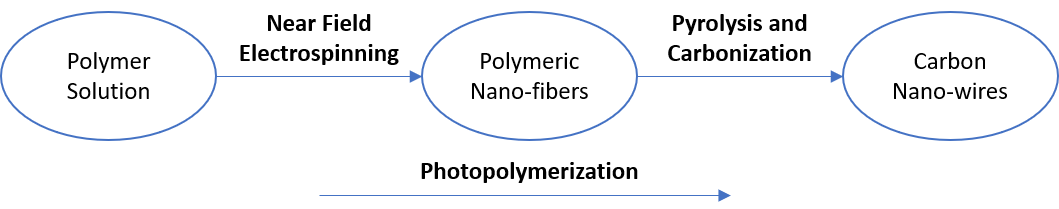
\includegraphics[width=0.95\textwidth]{./Figures/FabricationProcess.png}
%\decoRule
%\caption[Carbon Nano-wires Fabrication Process]{Fabrication process of carbon nano-wires to achieve through the proposed dissertation.}
%\label{fig:fabricationFlowChart}
%\end{figure}

%\begin{equation}
%\left(\tau _t^e-\frac{\tau _n^e \text{dr}}{\text{dz}}\right) 2 \pi  r+\frac{d \left(\pi  r^2
%   \left(\tau _{\text{zz}}-p\right)\right)}{\text{dz}}+\frac{\gamma  \text{dr} 2 \pi  r}{r
%   \text{dz}}+\rho  g \pi  r^2=\frac{d \left(\rho  \pi  r^2 v^2\right)}{\text{dz}}
%\label{eq:linearMomentum}
%\end{equation}